\chapter{Testy i wyniki}
\label{cha5}

W tym rozdziale zostały przedstawione wszystkie wykonane badania wraz z ich wynikami. W badaniach zostały uwzględnione wszystkie metody uczenia maszynowego przedstawione w rozdziale \ref{cha:ucz.masz} rozszerzając podejścia przytoczone w przeglądzie literatury (rozdział \ref{cha:stan.badan}). Badania te stanowią uzupełnienie i rozszerzenie prac z \cite{Reczek21}. 

\section{Opis podejścia}
\label{opis_podejścia}
%  (czym się różni od tego z rozdz. 2)
W pierwszej kolejności wykorzystano momenty Hu w celu wyłuskania z obrazów cech, za pomocą których można byłoby przeprowadzić klasyfikację. Analogicznie przetestowano tekstury Haralicka. Następnie liczby te podawano na wejście klasycznych klasyfikatorów. Kolejne testy objęły uogólnioną transformatę Hougha. Po zakończeniu tych testów rozpoczęto badania nad bardziej skomplikowanymi metodami. Przede wszystkim zdecydowano, aby rozpoznawać jakość zdjęć na podstawie liczby struktur różnych klas na obrazach. Szczegóły dotyczące wycinania, tworzenia bazy danych i rozpoznawania tych struktur zostały przedstawione w rozdziale \ref{}. W tym celu wykorzystano również wszystkie klasyfikatory klasyczne przedstawione w rozdziale \ref{cha:Wykorzystane metody uczenia maszynowego}. Wyniki porównano uwzględniając wiele aspektów, jak interpretowalność wyników, łatwość implementacji, prostotę algorytmu czy czas uczenia. Aby mieć ogląd całej sytuacji przetestowano również najskuteczniejsze obecnie architektury sieci neuronowych wykorzystywanych w celach klasyfikacji obrazów i również zostały one porównane wielopłaszczyznowo z pozostałymi wynikami. 

% ############ Klasyfikacja struktur i ocena jakości odlewów #############
\section{Klasyfikacja struktur i ocena jakości odlewów}
\label{sec:klasyfikacja_struktur}

Jest to najszerszy obszar badań, ponieważ dzięki danym w postaci zliczonych struktur można sprawdzić, czy kształty tych struktur mają wpływ na właściwości mechaniczne odlewów, a jeśli tak, to w jakim stopniu. Jak wszyscy wiemy, sieci neuronowe, które odbierają obrazy w postaci pikseli jako dane wejściowe i zwracają wynik w postaci „tak” lub „nie” na pytanie, czy wytrzymałość na rozciąganie danej mikrostruktury jest duża (lub mała) są modelami „czarnej skrzynki”, co oznacza, że trudno zweryfikować, dlaczego model podjął jedną decyzję nad drugą. Wykorzystując jednak dane w postaci liczby struktur i ich klas, można pokusić się o zbudowanie interpretowalnego modelu.

% ############ Klasyfikacja struktur i ocena jakości odlewów #############
\subsection{Momenty Hu oraz tekstury Haralicka}
\label{sec:hu_haralick}

Pierwszym podejściem było wykorzystanie tekstur Haralicka i momentów Hu do zidentyfikowania struktur na zdjęciu. Implementacja metody momentów Hu została zaczerpnięta z pakietu \ita{opencv-python}, natomiast implementacja tekstur Haralicka została zaczerpnięta z modułu \ita{mahotas}. Może się wydawać, że użycie tych algorytmów jest poprawne i przyniesie pożądane rezultaty, ponieważ zostały zaprojektowane specjalnie do tego celu. Rysunek \ref{fig:mesh20} przedstawia dwa zdjęcia różnych mikrostruktur, które potencjalnie można zidentyfikować przy użyciu technik opisanych powyżej.
\begin{figure}[h]
	\centering
	\begin{subfigure}{0.47\textwidth}
	    \centering
	    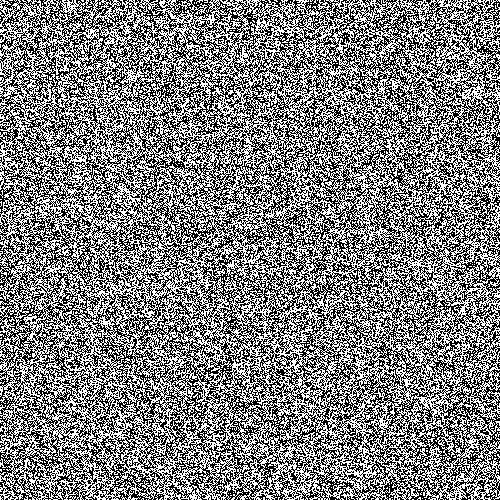
\includegraphics[width=1\textwidth]{rys.20.przyklad.mikrostruktur.a.png}
	    \subcaption{\label{subfigure_a}Zdjęcie mikrostruktury z obiektami klasy I (rys. \ref{fig:mesh14})}
	\end{subfigure}
	\begin{subfigure}{0.47\textwidth}
	    \centering
	    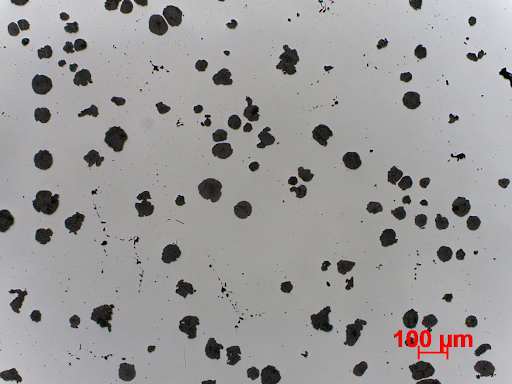
\includegraphics[width=1\textwidth]{rys.20.przyklad.mikrostruktur.b.png}
	    \subcaption{\label{subfigure_b}Zdjęcie mikrostruktury z obiektami klasy V (rys. \ref{fig:mesh14})}
	\end{subfigure}
	\caption{\label{fig:mesh20}Dwa przykładowe zdjęcia mikrostruktur. Ich tekstury i znajdujące się tam kształty diametralnie się różnią. Źródło: \cite{Pirowski17}}
\end{figure}
W pierwszym eksperymencie wykorzystano tekstury Haralicka, momenty Hu, a także modele maszyny wektorów nośnych (SVM) oraz lasów losowych (RF, RFC). 
\begin{table}[h]
	\centering
	\begin{threeparttable}
		\caption{Wyniki klasyfikacji binarnej z użyciem klasycznych klasyfikatorów, z wykorzystaniem momentów Hu oraz tekstur Haralicka. Źródło: opracowanie własne}
		\label{hu_haralick_table}
		\begin{tabularx}{1\textwidth}{ |X|X|X|X| }
		  \hline
		  \textbf{Model} & \textbf{Typ wejścia} & \textbf{Wagi klas} & \textbf{Dokładność}\\

		  \hline
		  SVM & Hu\tnote{a} & — & 71.5\%\\

		  \hline
		  SVM & Haralick\tnote{b} & — & 71.5\%\\

		  \hline
		  SVM & Hu + Haralick\tnote{c} & — & 71.5\%\\

		  \hline
		  RFC & Hu & zrównoważone & 58\%\\

		  \hline
  		  RFC & Haralick & zrównoważone & 70\%\\
  		  
		  \hline
  		  RFC & Hu + Haralick & zrównoważone & 70.1\%\\
  		  
		  \hline
		\end{tabularx}
		\begin{tablenotes}
			\footnotesize
			\item[a] Momenty Hu wyliczone ze zdjęć (7 elementów).
			\item[b] Tekstury Haralicka wyznaczone ze zdjęć (13 elementów).
			\item[c] Konkatenacja wyników dwóch powyższych metod (20 elementów).
		\end{tablenotes}
	\end{threeparttable}
\end{table}
Testy zostały przeprowadzone na zbiorze danych klasyfikowanych ze względu na wytrzymałość na rozciąganie. Niestety taka konfiguracja modeli i metod nie przyniosła oczekiwanych rezultatów. Testy przeprowadzono z wykorzystaniem sprawdzianu krzyżowego (ang. \ita{cross-validation}), a dokładnie sprawdzian \ita{k}-krotny, w którym oryginalna próba jest dzielona na \ita{k} podzbiorów, po czym każdy z tych podzbiorów jest wykorzystywany jako zbiór testowy, gdzie w tym czasie wszystkie pozostałe są wykorzystywane jako zbiór trenignowy. Następnie te \ita{k} rezultatów jest uśrednianych. 
Wyniki zaprezentowano w tabeli \ref{hu_haralick_table}.
\begin{table}[h]
	\centering
	\begin{threeparttable}
		\caption{Wyniki klasyfikacji binarnej z użyciem klasycznych klasyfikatorów, z wykorzystaniem momentów Hu oraz tekstur Haralicka. Dodatkowo rozszerzono dwukrotnie liczbę zdjęć o niskiej odporności (augmentacja). Źródło: opracowanie własne}
		\label{hu_haralick_table_with_augmentation}
		\begin{tabularx}{1\textwidth}{ |X|X|X|X| }
		  \hline
		  \textbf{Model} & \textbf{Typ wejścia} & \textbf{Wagi klas} & \textbf{Dokładność}\\

		  \hline
		  SVM & Hu & — & 55.7\%\\

		  \hline
		  SVM & Haralick & — & 54.6\%\\

		  \hline
		  SVM & Hu + Haralick & — & 54.6\%\\

		  \hline
		  RFC & Hu & zrównoważone & 56.6\%\\

		  \hline
  		  RFC & Haralick & zrównoważone & 86\%\\
  		  
		  \hline
  		  RFC & Hu + Haralick & zrównoważone & 86\%\\
  		  
		  \hline
		\end{tabularx}
	\end{threeparttable}
\end{table}
Jak widzimy, wyniki dla większości tych metod wynoszą około 71\%. Nieco gorszy wynik w przypadku lasu losowego może wynikać z zastosowania zrównoważenia wag klas. Jednakże zbiór danych składa się z 3358 zdjęć o wysokiej wytrzymałości na rozciąganie oraz 1337 zdjęć o niskiej wytrzymałości na rozciąganie (patrz \ref{sec:normalizacja_przyblizenia}). A więc liczba zdjęć o wysokiej wytrzymałości stanowi dokładnie 71\% wszystkich danych, stąd klasyfikatory zamiast rzeczywiście rozpoznawać dane tak na prawdę mogą dopasowywać się do częstotliwości występowania zdjęć określonej klasy. Stąd przeprowadzono dodatkowe testy z wykorzystaniem augmentacji (patrz \ref{cha:cha3.4}, \ref{sec:augmentacja}). Konkretnie zastosowano metodę odbicia na mniej licznej klasie (a więc na zdjęciach o niskiej wytrzymałości), dzięki czemu stosunek liczby zdjęć o wysokiej wytrzymałości do liczby wszystkich zdjęć spadł z 71\% do 55.7\%. Wyniki po przeprowadzeniu augmentacji znajdują się w tab. \ref{hu_haralick_table_with_augmentation}.
\begin{table}[h]
	\centering
	\begin{threeparttable}
		\caption{Wyniki klasyfikacji binarnej z użyciem klasycznych klasyfikatorów, z wykorzystaniem momentów Hu oraz tekstur Haralicka. Dane dodatkowo zostały zaszumione, aby zapobiec nadmiernemu dopasowaniu się modelu do danych. Źródło: opracowanie własne}
		\label{hu_haralick_table_with_augmentation_and_noise}
		\begin{tabularx}{1\textwidth}{ |X|X|X|X| }
		  \hline
		  \textbf{Model} & \textbf{Typ wejścia} & \textbf{Wagi klas} & \textbf{Dokładność}\\

		  \hline
		  SVM & Hu & — & 55.7\%\\

		  \hline
		  SVM & Haralick & — & 55.5\%\\

		  \hline
		  SVM & Hu + Haralick & — & 55.5\%\\

		  \hline
		  RFC & Hu & zrównoważone & 51.6\%\\

		  \hline
  		  RFC & Haralick & zrównoważone & 72.2\%\\
  		  
		  \hline
  		  RFC & Hu + Haralick & zrównoważone & 72.6\%\\
  		  
		  \hline
		\end{tabularx}
	\end{threeparttable}
\end{table}
Dodatkowo, aby nie zwiększać sztucznie dokładności ze względu na podobieństwo danych wygenerowanych sztucznie i oryginalnych, postanowiono nałożyć szum na dane wygenerowane syntetycznie. Zdecydowano się na szum biały. Wyniki zostały przedstawione w tabeli \ref{hu_haralick_table_with_augmentation_and_noise}.

\noindent Porównując wyniki otrzymane w tych trzech eksperymentach można dojść z penwością do kilku wniosków. Po pierwsze, widać wyraźnie, że wyniki pomiędzy modelami drzew oraz maszyny wektorów znacząco się różnią. W pierwszym eksperymencie wyniki dla SVM są lepsze od 1 do nawet 12 punktów procentowych. W pozostałych dwóch eksperymentach wyniki dla SVM są znacznie gorsze od tych dla lasu losowego, w ekstremalnym przypadku aż o 30 punktów procentowych. Po drugie, można zauważyć, że w większości przypadków wyniki dla momentów Hu są najgorsze, co można wytłumaczyć tym, iż jest to najprostsza metoda. Natomiast widzimy również wpływ augmentacji danych, jak również zaszumienia danych. Można przyjąć, iż najbardziej wiarygodne wyniki otrzymaliśmy w trzecim eksperymencie, gdyż, przede wszystkim, skuteczność algorytmu nie pokrywa się ze stosunkiem liczebności klas, oraz wyniki nie różnią się między sobą w niewytłumaczalny sposób. Mimo wszystko, ciężko do końca ocenić co tak naprawdę wpłynęło na te wyniki. Dodatkowo to podejście ma bardzo niską interpretowalność, tzn. ciężko ocenić dlaczego model wybrał jedną decyzję, zamiast innej. Natomiast atutem tego podejścia jest czas wykonywania (czas uczenia modeli). Mimo ustawienia parametrów SVM na wiele iteracji, a także ustawienie stosunkowo dużej liczby drzew dla algorytmu lasu losowego, czas uczenia tych modeli jest rzędu kilkunastu sekund. Jak widzimy, już nawet najprostsze metody dają pewne pozytywne rezultaty, dlatego zdecydowano się na nieco bardziej złożoną strategię, która być może podniesie skuteczność.

\subsection{Uogólniona transformata Hougha}
\label{hough}

W kolejnym kroku postanowiono zbadać uogólnioną transformatę Hougha (ang. \ita{generalised Hough transform}, \bo{GHT}). Wykorzystano w tym celu otwartoźródłową bibliotekę \ita{general-hough}. 
\begin{figure}[h]
    \centering
    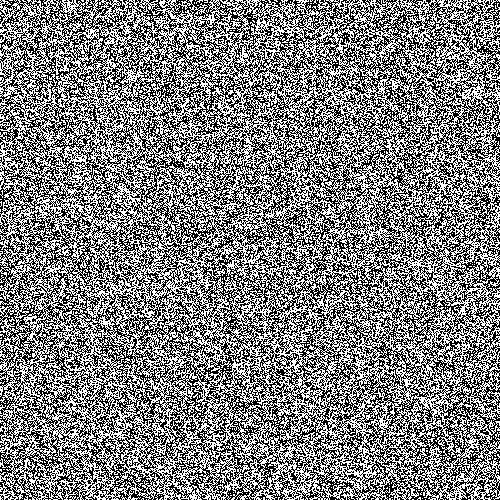
\includegraphics[width=0.6\textwidth]{rys.21.ght.duza.kulka.png}
    \caption{Wykrywanie kształtu przedstawionego na obrazie referencyjnym (ang. \ita{reference image}) na obrazie zapytania (ang. \ita{query image}). W prawym dolnym rogu na czerwono zaznaczono wykryte kształty. Żółty krzyżyk oznacza najtrafniejszy punkt. Obraz referencyjny w tym przypadku to czarne koło. Żródło: opracowanie własne przy wykorzystaniu biblioteki \ita{general-hough}}
    \label{fig:mesh21}
\end{figure}
Ta strategia jest bardziej skoncentrowana na pojedynczych strukturach i ich detekcji. Początkowe zmagania pokazały, że znajdowanie pojedynczych struktur danej klasy z pomocą tej metody jest możliwe, aczkolwiek nie wszystkie kształty, a niekiedy zdarzają się nawet większe pomyłki, co przedstawiono na poniższych obrazkach (rys. \ref{fig:mesh21}, \ref{fig:mesh22} i \ref{fig:mesh23}). Chociaż uważa się, że GHT ma zalety, takie jak:
\begin{itemize}
	\item odporność na częściowe lub nieznaczne zniekształcenie formy (tj. odporność na rozpoznanie pod okluzją), 
	\item odporność na obecnoć innych struktur na obrazie,
	\item odporność na szum,
	\item możliwość znajdowania wielu wystąpień danego kształtu na obrazie wejściowym.
\end{itemize}
Pomimo tego, że metoda ta została stworzona właśnie do rozpoznawania form zdefiniowanych matematycznie (takie występują na naszych obrazach), jego działanie nie spełniło naszych oczekiwań.
\begin{figure}[h]
    \centering
    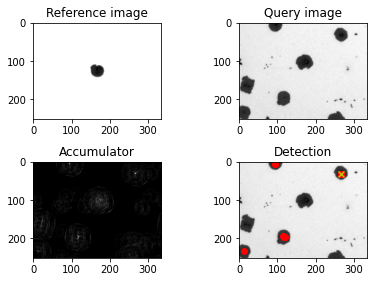
\includegraphics[width=0.6\textwidth]{rys.22.ght.mala.kulka.png}
    \caption{Działanie metody GHT na tym samym obrazie zapytania, lecz jako obraz referencyjny została użyta rzeczywista struktura znajdująca się na jednym ze zdjęć. Dodatkowo skala tej struktury jest taka sama, jak skala struktur na obrazie zapytania. Żródło: opracowanie własne przy wykorzystaniu biblioteki \ita{general-hough}}
    \label{fig:mesh22}
\end{figure}
Jak widać na rysunku \ref{fig:mesh21}, w oczy rzucają się dwa problemy. Po pierwsze, nie wykryto wszystkich kształtów. Po drugie, czerwone kropki oznaczające wykryty kształt niekiedy znajdują się na szarym tle, zamiast na czarnym kształcie. Ale to nie jedyne problemy. Zdarza się również, iż dana struktura jest oznaczona wielokrotnie. Dlatego zdecydowano się poeksperymentować z obrazami referencyjnymi, co potencjalnie może poprawić wyniki. Na kolejnym rysunku \ref{fig:mesh22} możemy zauważyć, że obraz zapytania jest wciąż ten sam, natomiast zmienił się obraz referencyjny. Tym razem jest to rzeczywista struktura, a więc nie jest ani idealnia czarna, ani idealnie okragła. Dodatkowo jej skala jest taka sama, jak skala struktur na obrazie zapytania. Możemy również zaobserwować na obrazie z wykrytymi kształtami (ang. \ita{detection}), iż tym razem czerwone kropki są rozmieszczone o wiele bardziej precyzyjne. 
\begin{figure}[h]
    \centering
    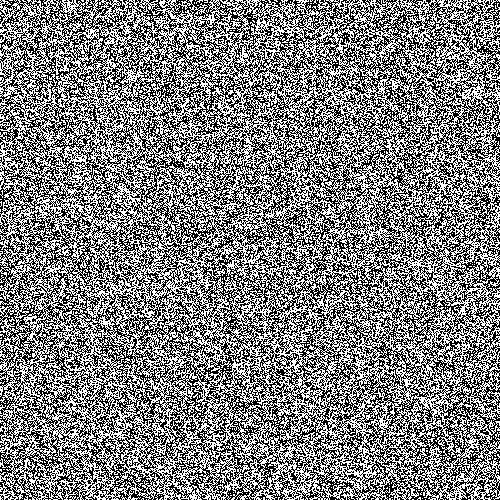
\includegraphics[width=0.6\textwidth]{rys.23.ght.mala.kulka.bez.szarosci.png}
    \caption{Kolejny test z tym samym obrazem zapytania, a także z tym samym obrazem referencyjnym, co na rys. \ref{fig:mesh22}. Widzimy, że metoda zadziałała jeszcze lepiej, gdyż wykryła poprawnie jeszcze jedną strukturę. Żródło: opracowanie własne przy wykorzystaniu biblioteki \ita{general-hough}}
    \label{fig:mesh23}
\end{figure}
Jednakże wciąż metoda ta nie jest na wystarczająco dokładna. W kolejnych testach usunięto dodatkowo szare tło z obrazów zapytania, przez co szare struktury znalazły się po tych przekształceniach na białym tle. Przykładowe wyniki zostały zaprezentowane na obrazie \ref{fig:mesh23}. Możemy zauważyć, że ten zabieg przyniósł oczekiwane efekty, a mianowicie wykryto poprawnie o jeden kształt więcej, niż przed tym zabiegiem.
Mimo wszystko takie podejście jest mało praktyczne, gdyż dla różnych obrazów należałoby dobierać obrazki referencyjne zgodnie ze skalą struktur na obrazach. Dodatkowo, pomimo tego, iż jest zaledwie sześć klas tych struktur, potrzebowalibymy znacznie więcej przykładów, aby pokryć przypadki, w których struktura jest zniekształcona, bądź nakłada się z inną strukturą. A więc wiemy już, że ta metoda nie może zostać wykorzystana w dalszych badaniach, a zatem należy wrócić do poszukiwań tej odpowiedniej metody.

\subsection{Detekcja krawędzi filtrem Canny'ego}
\label{canny}

Kolejne techniki były bardziej skoncentrowane na wycinaniu poszczególnych struktur, a następnie kategoryzowaniu każdej z nich niezależnie w kolejnych fazach. W tym celu wykorzystano pakiet \ita{opencv-python} (nazywana dalej \ita{cv}). Jednak w pierwszym kroku opracowano algorytm do przeprowadzania prostego zliczania struktur bez rozróżniania klasy kształtu. Krawędzie struktur wykrywano metodą Canny'ego \cite{Canny86}. Dodatkowo przetestowano różne techniki rozmywania obrazu (ang. \ita{blur}), czy inaczej – wygładzania, m.in. uśrednianie (w pythonie \ita{cv.blur}), rozmycie gaussowskie (ang. \ita{Gaussian blur}, w pythonie \ita{cv.GaussianBlur}), rozmycie środkowe (ang. \ita{median blurring}, w pythonie \ita{cv.medianBlur}) i filtrowanie dwustronne (ang. \ita{bilateral filtering}, w pythonie \ita{cv.bilateralFilter}). 
Otrzymujemy zróżnicowaną oprawę graficzną i efekty w zależności od rozmiaru jądra użytego w rozmyciu. Rysunek 22 przedstawia trzy zdjęcia, z których jeden jest oryginalny, a dwa inne, na których zastosowano wykrywanie krawędzi. Jeden ma antyaliasing (rozmiar jądra 5x5), podczas gdy drugi nie.
% chyba bym się w sumie nie trzymał tego schematu, tylko chronologicznie i jednoczesnie Rm i Rp ;d
%5.2. Opis wykonanych badań i testów oraz własnej implementacji
%
%5.3. Omówienie wyników uzyskanych za pomocą metod klasycznych
%
%5.3.1. Analiza wytrzymałości na rozciąganie
%
%5.3.2. Analiza granicy plastyczności
%
%5.4. Omówienie wyników uzyskanych za pomocą sieci neuronowych
%
%5.4.1. Analiza wytrzymałości na rozciąganie
%
%5.4.2. Analiza granicy plastyczności
%
%5.5. Omówienie wyników / całościowe
